\documentclass[aspectratio=169]{beamer}

% ============================================================
% Hybrid Quantum AI for Multiphysics Simulation -- seminar deck
% Simple Madrid style, ~33 frames.
%
% IMAGES: no image is embedded directly. Each figure uses \figbox{name}{w}{h}{caption}.
% If images/<name>.png exists it is inserted; otherwise a dashed placeholder
% showing the expected file name is drawn. Drop PNGs into images/ and recompile.
% ============================================================

\usetheme{Madrid}
\usecolortheme{seahorse}

\usepackage[utf8]{inputenc}
\usepackage[T1]{fontenc}
\usepackage{lmodern}
\usepackage{amsmath,amssymb}
\usepackage{booktabs}
\usepackage{array}
\usepackage{tabularx}
\usepackage{graphicx}
\usepackage[export]{adjustbox}
\usepackage{xcolor}
\usepackage{tikz}
\usetikzlibrary{arrows.meta,positioning,calc,decorations.pathreplacing}
\graphicspath{{images/}}

\setbeamertemplate{navigation symbols}{}
\setbeamertemplate{footline}[frame number]

\definecolor{qpurple}{HTML}{6B4C9A}
\definecolor{cblue}{HTML}{2C6E9E}
\definecolor{okgreen}{HTML}{2E7D4F}
\definecolor{warnorange}{HTML}{C9731C}
\definecolor{phgray}{HTML}{6E7780}
\definecolor{phfill}{HTML}{F2F4F6}

% Equation that shrinks only if wider than the text
\newcommand{\eq}[1]{\[\adjustbox{max width=0.94\linewidth}{$\displaystyle #1$}\]}

% Status tags
\newcommand{\shown}{\textcolor{okgreen}{\textbf{Shown}}}
\newcommand{\pending}{\textcolor{warnorange}{\textbf{In progress}}}
\newcommand{\planned}{\textcolor{phgray}{\textbf{Planned}}}

% \figbox{file-name-without-.png}{width}{height}{short description}
\newcommand{\figbox}[4]{%
  \IfFileExists{images/#1.png}{%
    \includegraphics[width=#2,height=#3,keepaspectratio]{images/#1.png}%
  }{%
    \begin{tikzpicture}
      \node[draw=phgray,dashed,thick,fill=phfill,minimum width=#2-1pt,minimum height=#3,
            align=center,text=phgray,font=\scriptsize,inner sep=3pt,text width=#2-9pt]
        {\textbf{[IMAGE PLACEHOLDER]}\\[1pt]\texttt{images/#1.png}\\[1pt]\textit{#4}};
    \end{tikzpicture}%
  }%
}

\title[Hybrid Quantum AI for Multiphysics]{Hybrid Quantum AI for Accelerating\\Multiphysics Simulation}
\subtitle{A Hybrid-QPINN / QPINO framework: Fourier features, data re-uploading\\and shallow parameterised quantum circuits}
\author{Aswin}
\date{October 2026}

\begin{document}

% =====================================================================
\begin{frame}
\titlepage
\end{frame}

\begin{frame}{Outline}
\tableofcontents
\end{frame}

% =====================================================================
\section{Motivation}
% =====================================================================

\begin{frame}{Accurate multiphysics simulation is too slow for design loops}
\begin{columns}[T,onlytextwidth]
\column{0.52\textwidth}
\begin{itemize}\small
  \item High-fidelity coupled CFD (flow + heat + rotation + phase change) takes hours to days per run.
  \item The real cost is the \textbf{parameter sweep}: every operating point is a new simulation.
  \item Process control and digital twins need full fields in \textbf{milliseconds}.
  \item Classical surrogates (PINN, PINO) help, but hit training bottlenecks on sharp, strongly coupled fields.
\end{itemize}
\vspace{0.1cm}
\begin{block}{Goal}
\small A surrogate that keeps the governing physics, generalises across operating conditions, and evaluates in real time.
\end{block}
\column{0.44\textwidth}
\centering
\figbox{cz-process-schematic}{\linewidth}{4.0cm}{Czochralski furnace schematic: crucible, melt, rotating crystal, heater}
\end{columns}
\end{frame}

\begin{frame}{Two industrial use cases}
\begin{columns}[T,onlytextwidth]
\column{0.48\textwidth}
\begin{block}{Silicon crystal growth (Czochralski)}
\begin{itemize}\small
  \item Seed crystal pulled from molten Si in a rotating crucible, 1685--1750\,K.
  \item Melt convection, swirl and thermal structure set defect density and oxygen uptake.
  \item \textbf{Aim:} fast field prediction to reduce defect formation.
\end{itemize}
\end{block}
\centering
\figbox{cz-melt-fields}{0.9\linewidth}{2.3cm}{CZ melt temperature / velocity field}
\column{0.48\textwidth}
\begin{block}{LH$_2$ cryogenic boil-off}
\begin{itemize}\small
  \item Heat leak into liquid-hydrogen tanks drives natural convection, stratification and evaporation.
  \item Turbulent convection with phase change and a moving liquid--vapour interface.
  \item \textbf{Aim:} predict boil-off rate and pressure rise for tank design.
\end{itemize}
\end{block}
\centering
\figbox{lh2-tank-schematic}{0.9\linewidth}{2.3cm}{LH$_2$ tank: heat leak, stratified layer, ullage vapour}
\end{columns}
\end{frame}

\begin{frame}{Our proposal in one slide}
\begin{enumerate}\setlength{\itemsep}{4pt}
  \item \textbf{Problem:} classical PINNs suffer from spectral bias, loss imbalance and badly scaled coupled fields.
  \item \textbf{Framework:} Hybrid-QPINN / QPINO, a classical network with a shallow parameterised quantum circuit (PQC) as a trainable feature map, fed by Fourier features and data re-uploading.
  \item \textbf{Target physics:} strongly coupled non-linear transport: velocity, temperature, and (next) concentration and evolving interfaces.
  \item \textbf{Benchmarks:} silicon CZ growth (running) and LH$_2$ boil-off (defined).
  \item \textbf{Destination:} real-time digital twins and fast parametric exploration.
\end{enumerate}
\vspace{0.2cm}
\begin{alertblock}{How to read the results}
Each claim in this talk carries a status: \shown{} (measured), \pending{} (experiment running or partially done), or \planned{}.
\end{alertblock}
\end{frame}

% =====================================================================
\section{Why classical PINNs struggle}
% =====================================================================

\begin{frame}{Physics-informed neural networks in one slide}
\begin{columns}[T,onlytextwidth]
\column{0.55\textwidth}
\begin{itemize}
  \item A network $\hat u_\theta(x)$ is trained so that the PDEs and boundary/initial conditions hold.
  \item Derivatives come from automatic differentiation: no mesh, no stencil.
\end{itemize}
\eq{\mathcal{L} = \mathcal{L}_{\mathrm{data}} + \lambda_{\mathrm{PDE}}\,\mathcal{L}_{\mathrm{PDE}} + \lambda_{\mathrm{BC}}\,\mathcal{L}_{\mathrm{BC}} + \lambda_{\mathrm{IC}}\,\mathcal{L}_{\mathrm{IC}}}
\begin{itemize}
  \item Strength: little labelled data, natural fit for coupled equations.
  \item Limitation: one PINN = one parameter setting. Neural operators (PINO) learn whole solution families.
\end{itemize}
\column{0.41\textwidth}
\centering
\figbox{pinn-concept}{\linewidth}{4.2cm}{PINN: coordinates $\to$ network $\to$ fields; autodiff residuals in the loss}
\end{columns}
\end{frame}

\begin{frame}{Bottleneck 1: spectral bias}
\begin{columns}[T,onlytextwidth]
\column{0.55\textwidth}
\begin{itemize}
  \item MLPs learn low frequencies first; high-frequency content converges slowly (Rahaman et al., 2019).
  \item Coupled transport fields are full of sharp structure: thermal boundary layers, wall shear, swirl near rotating walls, phase interfaces.
  \item Classical remedy: Fourier feature mapping of the inputs (Tancik et al., 2020).
  \item \textbf{Our addition:} a second, \emph{trainable} non-linear feature map, the PQC, whose outputs are trigonometric polynomials of its inputs.
\end{itemize}
\column{0.41\textwidth}
\centering
\figbox{spectral-bias-illustration}{\linewidth}{4.0cm}{Low- vs high-frequency fit over training epochs (illustrative)}
\end{columns}
\end{frame}

\begin{frame}{Bottleneck 2: loss-term imbalance}
\begin{itemize}
  \item The loss term with the largest raw gradient dominates the update (Wang et al., 2021).
  \item A small \emph{total} loss can hide poor boundary satisfaction and a wrong field.
\end{itemize}
\vspace{0.1cm}
\begin{center}
\small
\begin{tabular}{lccc}
\toprule
Trainer (1D heat equation) & PDE loss & BC/IC loss & Rel.\ $L_2$ error \\
\midrule
Fixed weights            & $3.96\times10^{-3}$ & $1.15\times10^{-3}$ & $0.084$ \\
Normalised gradients     & $9.74\times10^{-3}$ & $9.05\times10^{-4}$ & $\mathbf{0.054}$ \\
Adaptive weights         & $\mathbf{8.22\times10^{-7}}$ & $2.00\times10^{-1}$ & $1.368$ \\
\bottomrule
\end{tabular}
\end{center}
\vspace{0.1cm}
\begin{block}{Lesson carried into this work}
The smallest PDE residual gave the worst solution. We report loss components and per-field errors, never only a weighted total.
\end{block}
\smallskip
{\scriptsize Chapagain et al., NeurIPS 2026 Sim2Science workshop.}
\end{frame}

\begin{frame}{Bottleneck 3: scale mismatch between coupled fields}
\begin{columns}[T,onlytextwidth]
\column{0.55\textwidth}
\begin{itemize}
  \item Five coupled outputs: $u_r, u_z, u_\theta, p, T$, with very different magnitudes.
  \item In the CZ model the pressure coefficient is
  \[p_{\mathrm{coeff}} = \frac{p_{\mathrm{scale}}}{v_{\mathrm{scale}}^2} = 134{,}128.\]
  \item Viscous terms scale as $1/Re \approx 0.067$.
  \item Pressure-to-viscous ratio $\approx 2\times10^{6}:1$.
\end{itemize}
\column{0.41\textwidth}
\begin{alertblock}{Consequence}
The pressure residual can overwhelm the data signal during physics-informed training. This is the main stability issue we measured (see Results).
\end{alertblock}
\vspace{0.2cm}
\begin{block}{Design response}
Hard constraints, staged physics warm-up, EMA residual balancing, and (next) per-field residual scaling.
\end{block}
\end{columns}
\end{frame}

% =====================================================================
\section{The Hybrid-QPINN / QPINO framework}
% =====================================================================

\begin{frame}{Architecture overview}
\centering
\resizebox{\linewidth}{!}{%
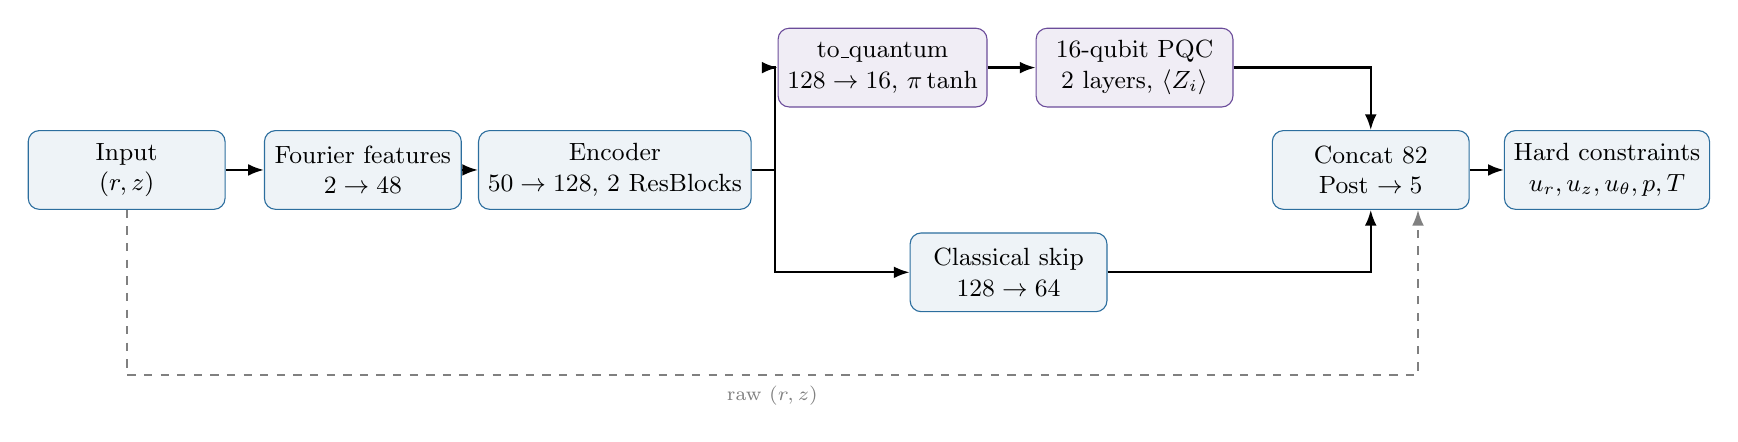
\begin{tikzpicture}[
  font=\small,
  cls/.style={rounded corners,draw=cblue,fill=cblue!8,minimum height=1.0cm,minimum width=2.5cm,align=center},
  qnt/.style={rounded corners,draw=qpurple,fill=qpurple!10,minimum height=1.0cm,minimum width=2.5cm,align=center},
  arr/.style={-{Latex[length=2mm]},thick}
]
\node[cls] (in) at (0,0) {Input\\$(r,z)$};
\node[cls] (ff) at (3.0,0) {Fourier features\\$2\to48$};
\node[cls] (enc) at (6.2,0) {Encoder\\$50\to128$, 2 ResBlocks};
\node[qnt] (tq) at (9.6,1.3) {to\_quantum\\$128\to16$, $\pi\tanh$};
\node[qnt] (pqc) at (12.8,1.3) {16-qubit PQC\\2 layers, $\langle Z_i\rangle$};
\node[cls] (sk) at (11.2,-1.3) {Classical skip\\$128\to64$};
\node[cls] (post) at (15.8,0) {Concat 82\\Post $\to5$};
\node[cls] (out) at (18.8,0) {Hard constraints\\$u_r,u_z,u_\theta,p,T$};
\draw[arr] (in)--(ff); \draw[arr] (ff)--(enc);
\draw[arr] (enc.east)--++(0.3,0)|-(tq.west);
\draw[arr] (enc.east)--++(0.3,0)|-(sk.west);
\draw[arr] (tq)--(pqc);
\draw[arr] (pqc.east)-|(post.north);
\draw[arr] (sk.east)-|(post.south);
\draw[arr] (post)--(out);
\draw[arr,dashed,gray] (in.south)--++(0,-2.1)-|node[pos=0.25,below,font=\scriptsize]{raw $(r,z)$} ([xshift=0.6cm]post.south);
\end{tikzpicture}}

\vspace{0.3cm}
\begin{columns}[T,onlytextwidth]
\column{0.32\textwidth}
\begin{block}{Classical backbone}
\footnotesize Fourier encoding plus residual MLP: carries most of the computation.
\end{block}
\column{0.32\textwidth}
\begin{exampleblock}{Quantum feature map}
\footnotesize 16 qubits, 2 layers, 96 trainable angles; 16 expectation values out.
\end{exampleblock}
\column{0.32\textwidth}
\begin{block}{Skip path}
\footnotesize Guarantees the head never depends solely on the quantum bottleneck.
\end{block}
\end{columns}
\end{frame}

\begin{frame}{Ingredient 1: Fourier feature mapping}
\begin{columns}[T,onlytextwidth]
\column{0.52\textwidth}
\begin{itemize}
  \item Frozen random matrix $B\in\mathbb{R}^{2\times24}$, $B_{ij}\sim\mathcal{N}(0,6^2)$.
  \eq{\gamma(x) = \big[\sin(2\pi\,xB),\ \cos(2\pi\,xB)\big]\in\mathbb{R}^{48}}
  \item Frequencies span roughly $\pm15$ cycles per unit length in normalised coordinates.
  \item Concatenated with raw $(r,z)$: 50 inputs to the encoder.
  \item Gives the network high-frequency access from the first layer, at zero trainable cost.
\end{itemize}
\column{0.44\textwidth}
\centering
\figbox{fourier-B-matrix}{\linewidth}{3.4cm}{Fourier feature frequencies, $B$ matrix ($2\times24$) heatmap}
\end{columns}
\end{frame}

\begin{frame}{Ingredient 2: shallow parameterised quantum circuit}
\centering
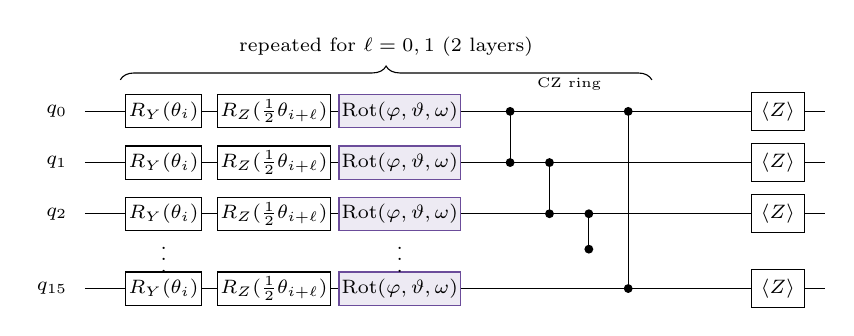
\begin{tikzpicture}[
  font=\scriptsize,
  g/.style={draw,fill=white,minimum width=0.95cm,minimum height=0.42cm,inner sep=1pt},
  gq/.style={draw=qpurple,fill=qpurple!12,minimum width=1.25cm,minimum height=0.42cm,inner sep=1pt}
]
\foreach \y/\lab in {0/{$q_0$},-0.65/{$q_1$},-1.3/{$q_2$},-2.25/{$q_{15}$}}{
  \node[anchor=east] at (-0.1,\y) {\lab};
  \draw (0,\y)--(9.4,\y);
  \node[g] at (1.0,\y) {$R_Y(\theta_i)$};
  \node[g] at (2.4,\y) {$R_Z(\tfrac12\theta_{i+\ell})$};
  \node[gq] at (4.0,\y) {Rot$(\varphi,\vartheta,\omega)$};
  \node[draw,fill=white,minimum width=0.6cm,minimum height=0.42cm] at (8.8,\y) {$\langle Z\rangle$};
}
\node at (1.0,-1.78) {$\vdots$}; \node at (4.0,-1.78) {$\vdots$};
% CZ ring
\foreach \ya/\yb/\x in {0/-0.65/5.4,-0.65/-1.3/5.9,-1.3/-1.75/6.4}{
  \draw (\x,\ya)--(\x,\yb); \fill (\x,\ya) circle (1.6pt); \fill (\x,\yb) circle (1.6pt);
}
\draw (6.9,0)--(6.9,-2.25); \fill (6.9,0) circle (1.6pt); \fill (6.9,-2.25) circle (1.6pt);
\node[font=\tiny] at (6.15,0.35) {CZ ring};
\draw[decorate,decoration={brace,amplitude=5pt}] (0.45,0.4)--(7.2,0.4)
  node[midway,above=5pt] {repeated for $\ell = 0,1$ (2 layers)};
\end{tikzpicture}

\vspace{0.25cm}
\begin{columns}[T,onlytextwidth]
\column{0.5\textwidth}
\begin{enumerate}\small
  \item Encode: $R_Y(\theta_i)$, $\theta_i=\pi\tanh(h_i)\in[-\pi,\pi]$.
  \item Re-upload: $R_Z(0.5\,\theta_{(i+\ell)\bmod16})$.
  \item Train: $\mathrm{Rot}(\varphi_i,\vartheta_i,\omega_i)$, 48 angles/layer.
  \item Entangle: CZ ring, closing $q_{15}$--$q_0$.
\end{enumerate}
\column{0.46\textwidth}
\begin{block}{Readout}
\small $\langle Z_i\rangle$, $i=0,\dots,15$ $\to$ LayerNorm(16).\\
\textbf{96 trainable quantum parameters}, about 50 gates per shot on hardware.
\end{block}
\end{columns}
\end{frame}

\begin{frame}{Ingredient 3: data re-uploading}
\begin{columns}[T,onlytextwidth]
\column{0.55\textwidth}
\begin{itemize}
  \item A circuit that encodes its input once realises only a low-degree Fourier series of that input.
  \item Re-uploading the data in every layer raises the accessible frequency spectrum (P\'erez-Salinas et al., 2020; Schuld et al., 2021).
  \item The cyclic shift $\theta_{(i+\ell)\bmod16}$ lets each layer mix a different combination of latent features.
  \item Together with Fourier inputs, this targets the high-frequency content that spectral bias suppresses.
\end{itemize}
\column{0.41\textwidth}
\begin{exampleblock}{Design rule}
The PQC is a compact, expressive \emph{feature extractor}. The classical network carries the bulk of the computation, which keeps the circuit shallow enough for today's hardware.
\end{exampleblock}
\end{columns}
\end{frame}

\begin{frame}{Parameter budget: a deliberately small quantum layer}
\begin{columns}[T,onlytextwidth]
\column{0.5\textwidth}
\begin{center}
\small
\begin{tabular}{lr}
\toprule
Component & Parameters \\
\midrule
Coordinate projector & 23,040 \\
ResidualMLP blocks ($2\times2$) & 66,048 \\
to\_quantum & 9,296 \\
Classical skip & 8,256 \\
\textbf{Quantum circuit} & \textbf{96} \\
Quantum LayerNorm & 32 \\
Post network & 19,205 \\
Fourier $B$ (frozen) & 48 \\
\midrule
\textbf{Total} & \textbf{126,021} \\
\bottomrule
\end{tabular}
\end{center}
\column{0.46\textwidth}
\begin{block}{Why small?}
\small
\begin{itemize}
  \item Shallow circuits survive NISQ noise.
  \item Few angles $\Rightarrow$ cheap hardware fine-tuning.
  \item 0.076\% of all parameters.
\end{itemize}
\end{block}
\begin{alertblock}{Consequence for evaluation}
\small Any gain must be attributed to the PQC by a controlled ablation, not assumed.
\end{alertblock}
\end{columns}
\end{frame}

\begin{frame}{Governing equations (1/2): mass and momentum}
Steady, axisymmetric, incompressible Navier--Stokes with Boussinesq buoyancy (nondimensional).

\textbf{Continuity:}
\eq{\frac{\partial (r\,u_r)}{\partial r} + r\,\frac{\partial u_z}{\partial z} = 0}
\textbf{Radial momentum:}
\eq{u_r u_{r,r} + u_z u_{r,z} - \frac{u_\theta^2}{r} + p_{\mathrm{coeff}}\,p_{,r} - \frac{1}{Re}\Big[u_{r,rr} + \frac{u_{r,r}}{r} - \frac{u_r}{r^2} + u_{r,zz}\Big] = 0}
\textbf{Axial momentum:}
\eq{u_r u_{z,r} + u_z u_{z,z} + p_{\mathrm{coeff}}\,p_{,z} - \frac{1}{Re}\Big[u_{z,rr} + \frac{u_{z,r}}{r} + u_{z,zz}\Big] - \frac{Gr}{Re^2}\,\theta = 0}
\end{frame}

\begin{frame}{Governing equations (2/2): swirl and energy}
\textbf{Swirl (angular momentum):}
\eq{u_r u_{\theta,r} + u_z u_{\theta,z} + \frac{u_r u_\theta}{r} - \frac{1}{Re}\Big[u_{\theta,rr} + \frac{u_{\theta,r}}{r} - \frac{u_\theta}{r^2} + u_{\theta,zz}\Big] = 0}
\textbf{Energy:}
\eq{u_r \theta_{,r} + u_z \theta_{,z} - \frac{1}{Pr\,Re}\Big[\theta_{,rr} + \frac{\theta_{,r}}{r} + \theta_{,zz}\Big] = 0}
\vspace{0.1cm}
\begin{center}
\small $\theta = \dfrac{T-T_{\min}}{T_{\max}-T_{\min}}$,\qquad $Re=15$,\quad $Pr=28.463$,\quad $Gr=8000$,\quad $p_{\mathrm{coeff}}=134{,}128$
\end{center}
\end{frame}

\begin{frame}{Physics loss and hard constraints}
\begin{columns}[T,onlytextwidth]
\column{0.55\textwidth}
\begin{itemize}\small
  \item Derivatives via \texttt{torch.autograd.grad}, \texttt{create\_graph=True} (second order).
  \item Five residuals (continuity, $r$, $z$, swirl, energy), balanced by EMA weighting, $\beta=0.95$.
  \item Staged schedule: data only until epoch 50, then physics weight ramped $0\to0.05$.
  \item Gradient clipping at L2 norm 1.0.
  \item \textbf{Hard constraints:} $u_r=r\cdot\mathrm{raw}_0$, $u_\theta=r\cdot\mathrm{raw}_2$, so both vanish on the axis exactly.
\end{itemize}
\column{0.41\textwidth}
\begin{alertblock}{Current limitation}
\small The PQC output is detached inside the physics loss, so PDE gradients do not reach the quantum angles. The PQC is currently shaped by the data loss only.
\end{alertblock}
\begin{block}{Fix in progress}
\small Parameter-shift or adjoint gradients for the residual path.
\end{block}
\end{columns}
\end{frame}

\begin{frame}{From QPINN to QPINO: learning across operating conditions}
\begin{columns}[T,onlytextwidth]
\column{0.52\textwidth}
\begin{block}{QPINN (today)}
\small One model per operating condition: $(r,z)\mapsto(u_r,u_z,u_\theta,p,T)$.
\end{block}
\begin{block}{QPINO (next)}
\small The process parameters become inputs:
\eq{(r,z,\,s)\ \mapsto\ (u_r,u_z,u_\theta,p,T),\quad s\in\{T_{\mathrm{hot}},\,\omega_c,\,\omega_s,\,v_{\mathrm{pull}}\}}
One trained surrogate serves the whole sweep: the basis for parametric exploration and digital twins.
\end{block}
\column{0.44\textwidth}
\centering
\figbox{qpino-concept}{\linewidth}{4.2cm}{QPINO: operating parameters $s$ enter the encoder alongside $(r,z)$; one model, many conditions}
\end{columns}
\end{frame}

% =====================================================================
\section{Benchmarks and protocol}
% =====================================================================

\begin{frame}{Benchmark 1: silicon CZ melt (running)}
\begin{columns}[T,onlytextwidth]
\column{0.42\textwidth}
\begin{center}
\small
\begin{tabular}{ll}
\toprule
Property & Value \\
\midrule
Reference & Axisymmetric CFD \\
Domain & $r,z\in[0,0.3]$\,m \\
Points & 18,108 \\
Outputs & $u_r,u_z,u_\theta,p,T$ \\
$T$ range & 1685--1750\,K \\
Split & 17,203 / 905 \\
\bottomrule
\end{tabular}
\end{center}
\begin{block}{Scope}
\footnotesize Steady, laminar, single-phase reference cases, not fully resolved industrial melt flow.
\end{block}
\column{0.56\textwidth}
\centering
\figbox{training-data-fields}{\linewidth}{2.4cm}{Training data fields (normalised): $u_r$, $u_z$, $u_\theta$, $p$, $T$ over $(r,z)$}
\vspace{0.2cm}
\begin{block}{Next physics}
\footnotesize Oxygen concentration transport (species equation) and the evolving melt--crystal interface.
\end{block}
\end{columns}
\end{frame}

\begin{frame}{Benchmark 2: LH$_2$ cryogenic boil-off (defined)}
\begin{columns}[T,onlytextwidth]
\column{0.55\textwidth}
\begin{block}{Physics to capture}
\begin{itemize}\small
  \item Wall heat leak $\to$ natural convection boundary layer and thermal stratification.
  \item Turbulent convection (RANS closure in the reference CFD).
  \item Liquid--vapour interface with evaporation (VOF + phase-change mass transfer).
  \item Outputs: velocity, temperature, phase fraction, boil-off rate, ullage pressure.
\end{itemize}
\end{block}
\begin{alertblock}{Status}
\small Benchmark and outputs defined; reference CFD data not yet generated. \planned
\end{alertblock}
\column{0.41\textwidth}
\centering
\figbox{lh2-boiloff-cfd}{\linewidth}{4.6cm}{LH$_2$ tank CFD: temperature stratification and interface (reference, to be generated)}
\end{columns}
\end{frame}

\begin{frame}{Evaluation protocol: what counts as evidence}
\begin{columns}[T,onlytextwidth]
\column{0.5\textwidth}
\begin{itemize}\small
  \item \textbf{Ablations:} (a) classical-only, matched parameter budget; (b) random-feature layer in place of the PQC.
  \item \textbf{Baselines:} classical PINN and PINO with matched optimiser, sampling, seeds, budget.
  \item \textbf{Generalisation:} case-wise holdout of a whole operating condition.
  \item \textbf{Reporting:} per-field error and unweighted loss components.
  \item \textbf{Cost:} wall time to target error and inference latency.
\end{itemize}
\column{0.46\textwidth}
\begin{center}
\small
\begin{tabular}{lll}
\toprule
Sweep & Range & Held out \\
\midrule
$T_{\mathrm{hot}}$ & 1730--1785\,K & 1780\,K \\
$\omega_c$ (crucible) & $-10$ to $-1$ rpm & $-4$ rpm \\
$\omega_s$ (crystal) & 4--20 rpm & 7 rpm \\
\bottomrule
\end{tabular}
\end{center}
\vspace{0.2cm}
\begin{block}{Why this matters}
\footnotesize A random spatial split measures interpolation. A held-out operating condition measures what a digital twin actually needs.
\end{block}
\end{columns}
\end{frame}

\begin{frame}{Compute pipeline: laptop $\to$ GPU $\to$ quantum hardware}
\centering
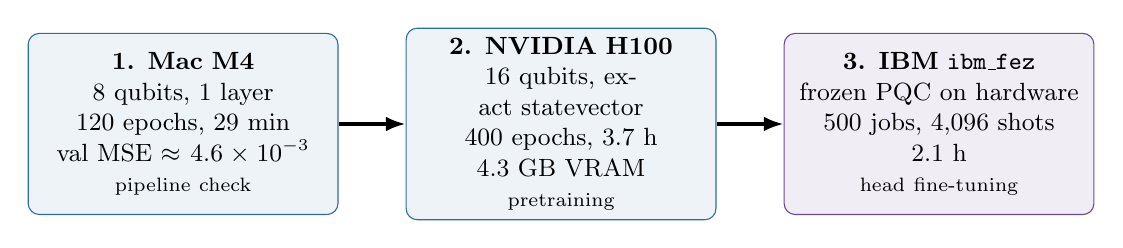
\begin{tikzpicture}[
  font=\small,
  st/.style={rounded corners,draw=cblue,fill=cblue!8,minimum width=3.9cm,minimum height=2.3cm,align=center,text width=3.7cm},
  sq/.style={rounded corners,draw=qpurple,fill=qpurple!10,minimum width=3.9cm,minimum height=2.3cm,align=center,text width=3.7cm},
  arr/.style={-{Latex[length=2.5mm]},very thick}
]
\node[st] (a) at (0,0) {\textbf{1. Mac M4}\\8 qubits, 1 layer\\120 epochs, 29 min\\val MSE $\approx4.6\times10^{-3}$\\\scriptsize pipeline check};
\node[st] (b) at (4.8,0) {\textbf{2. NVIDIA H100}\\16 qubits, exact statevector\\400 epochs, 3.7 h\\4.3 GB VRAM\\\scriptsize pretraining};
\node[sq] (c) at (9.6,0) {\textbf{3. IBM \texttt{ibm\_fez}}\\frozen PQC on hardware\\500 jobs, 4,096 shots\\2.1 h\\\scriptsize head fine-tuning};
\draw[arr] (a)--(b); \draw[arr] (b)--(c);
\end{tikzpicture}

\vspace{0.4cm}
\begin{block}{Note on simulation}
\small A 16-qubit circuit is a $2^{16}$-amplitude statevector: exactly simulable on one GPU. Hardware runs here test noise robustness and deployment, not quantum advantage.
\end{block}
\end{frame}

% =====================================================================
\section{Results}
% =====================================================================

\begin{frame}{Result 1: fast convergence in the data-driven phase \shown}
\begin{columns}[T,onlytextwidth]
\column{0.54\textwidth}
\begin{center}
\small
\begin{tabular}{llll}
\toprule
Epoch & Train loss & Val MSE & Val $T$ \\
\midrule
1  & $1.16\times10^{-2}$ & $4.83\times10^{-3}$ & $1.37\times10^{-3}$ \\
10 & $5.92\times10^{-5}$ & $3.11\times10^{-4}$ & $1.47\times10^{-4}$ \\
\textbf{20} & $\mathbf{5.26\times10^{-5}}$ & $\mathbf{1.58\times10^{-4}}$ & $\mathbf{5.07\times10^{-5}}$ \\
30 & $2.96\times10^{-5}$ & $1.75\times10^{-4}$ & $6.15\times10^{-5}$ \\
50 & $2.07\times10^{-5}$ & $2.13\times10^{-4}$ & $2.91\times10^{-5}$ \\
\bottomrule
\end{tabular}
\end{center}
\begin{block}{Reading}
\small Validation MSE drops 30$\times$ in 20 epochs. Best checkpoint: $\mathbf{1.58\times10^{-4}}$ (random spatial split).
\end{block}
\column{0.42\textwidth}
\centering
\figbox{training-curve-v2}{\linewidth}{4.4cm}{Train / validation loss vs epoch (H100 run, 400 epochs); physics ramp start marked at epoch 50}
\end{columns}
\end{frame}

\begin{frame}{Result 2: all five coupled fields captured \shown}
\begin{columns}[T,onlytextwidth]
\column{0.40\textwidth}
\begin{center}
\small
\begin{tabular}{lll}
\toprule
Field & Val MSE & \\
\midrule
$u_r$ & $1.93\times10^{-6}$ & excellent \\
$u_z$ & $5.78\times10^{-5}$ & very good \\
$u_\theta$ & $1.44\times10^{-6}$ & excellent \\
$p$ & $4.62\times10^{-5}$ & good \\
$T$ & $5.07\times10^{-5}$ & good \\
\bottomrule
\end{tabular}
\end{center}
\vspace{0.1cm}
{\footnotesize Best checkpoint (epoch 20), normalised fields, in distribution.}
\column{0.58\textwidth}
\centering
\figbox{parity-best-checkpoint}{\linewidth}{2.3cm}{Prediction vs ground truth per field, best checkpoint (parity plots)}
\vspace{0.15cm}
\figbox{field-error-maps}{\linewidth}{2.3cm}{Absolute error maps over $(r,z)$ for $u_r,u_z,u_\theta,p,T$}
\end{columns}
\end{frame}

\begin{frame}{Result 3: naive physics weighting destabilises training \shown}
\begin{columns}[T,onlytextwidth]
\column{0.52\textwidth}
\begin{center}
\small
\begin{tabular}{lllr}
\toprule
Field & Best (ep.\,20) & Final (ep.\,400) & Factor \\
\midrule
$u_r$ & $1.93\times10^{-6}$ & $1.79\times10^{-4}$ & 93$\times$ \\
$u_z$ & $5.78\times10^{-5}$ & $8.83\times10^{-3}$ & 153$\times$ \\
$u_\theta$ & $1.44\times10^{-6}$ & $5.06\times10^{-5}$ & 35$\times$ \\
$p$ & $4.62\times10^{-5}$ & $0.100$ & \textbf{2,165$\times$} \\
$T$ & $5.07\times10^{-5}$ & $0.129$ & \textbf{2,544$\times$} \\
\bottomrule
\end{tabular}
\end{center}
{\scriptsize\ttfamily
{[0280]} loss=1.04e+09 data=5.06e-02 phys=2.16e+10\\
{[0290]} loss=1.18e+14 data=4.97e-02 phys=2.15e+15\\
{[0300]} loss=5.57e-02 data=4.85e-02 phys=9.62e-02}
\column{0.44\textwidth}
\begin{alertblock}{Diagnosis}
\small Data loss stays near 0.05; the blow-up is entirely in the physics residual. Root cause: the $p_{\mathrm{coeff}}$ scale mismatch (Bottleneck 3).
\end{alertblock}
\begin{exampleblock}{Fixes under test \pending}
\small Physics weight 0.001--0.005; per-field pressure residual scaling; re-check pressure nondimensionalisation.
\end{exampleblock}
\end{columns}
\end{frame}

\begin{frame}{Result 4: end-to-end run on real quantum hardware \shown}
\begin{columns}[T,onlytextwidth]
\column{0.48\textwidth}
\begin{center}
\footnotesize
\begin{tabular}{ll}
\toprule
Metric & Value \\
\midrule
Backend & \texttt{ibm\_fez} (156 qubits) \\
Jobs completed / failed & \textbf{500 / 0} \\
Shots per job & 4,096 \\
Total shots & \textbf{2,048,000} \\
Session & 125 min, 4.0 jobs/min \\
Trainable scope & head only (19,205) \\
Calibration points & 8 \\
\bottomrule
\end{tabular}
\end{center}
{\footnotesize Session stopped by plan time at $\approx$62 of 100 planned epochs; all results stored under saved job IDs.}
\column{0.48\textwidth}
\centering
\figbox{calibration-coverage}{\linewidth}{3.6cm}{Calibration subset coverage: 8 points across the $(r,z)$ domain}
\end{columns}
\end{frame}

\begin{frame}{Hardware noise and why the head is fine-tuned}
\begin{columns}[T,onlytextwidth]
\column{0.44\textwidth}
\begin{center}
\small
\begin{tabular}{lrrr}
\toprule
Qubit & $\langle Z\rangle$ & $\sigma$ & $\sigma_{\mathrm{shot}}$ \\
\midrule
$Q_0$  & $+0.342$ & 0.012 & 0.015 \\
$Q_1$  & $+0.765$ & 0.014 & 0.010 \\
$Q_5$  & $-0.856$ & 0.009 & 0.008 \\
$Q_{13}$ & $-0.908$ & 0.007 & 0.007 \\
\bottomrule
\end{tabular}
\end{center}
{\scriptsize $\sigma_{\mathrm{shot}}=\sqrt{(1-\langle Z\rangle^2)/4096}$; reported spread is close to shot noise.}
\vspace{0.1cm}
\begin{block}{Adaptation strategy}
\footnotesize Freeze the PQC; retrain only the classical head on hardware $\langle Z_i\rangle$.
\end{block}
\column{0.54\textwidth}
\centering
\figbox{initial-predictions-before-finetune}{\linewidth}{2.3cm}{Initial predictions vs ground truth, before fine-tuning (near-constant outputs)}
\vspace{0.1cm}
\begin{alertblock}{Observation}
\footnotesize Before fine-tuning, predictions on hardware features are nearly flat across all five fields: the head must be re-adapted. Completing this run is the next hardware step.
\end{alertblock}
\end{columns}
\end{frame}

\begin{frame}{Inside the trained circuit}
\begin{columns}[T,onlytextwidth]
\column{0.5\textwidth}
\centering
\figbox{quantum-rot-params}{\linewidth}{3.0cm}{Rot gate angles $(\varphi,\vartheta,\omega)$ per qubit, layers 0 and 1}
\vspace{0.1cm}
\begin{itemize}\footnotesize
  \item Angles span the full $[0,2\pi]$ range (mean 3.49, std 1.79 rad).
  \item No qubit stuck at a degenerate value.
\end{itemize}
\column{0.48\textwidth}
\centering
\figbox{quantum-layernorm}{\linewidth}{2.3cm}{Quantum LayerNorm scale $\gamma$ and bias $\beta$ per qubit}
\vspace{0.1cm}
\begin{itemize}\footnotesize
  \item In the longer v1 run (650 epochs), LayerNorm weights qubits unequally ($\gamma\approx0.3$--$1.2$): the head learns to rely on some quantum features more than others.
  \item At the v2 best checkpoint (epoch 20) $\gamma$ is still near 1.
\end{itemize}
\end{columns}
\vspace{0.1cm}
\begin{block}{}
\centering\footnotesize The circuit is active and differentiated. Whether it adds accuracy is what the ablation will tell us.
\end{block}
\end{frame}

\begin{frame}{Benchmark program: convergence, generalisation, cost}
\begin{columns}[T,onlytextwidth]
\column{0.33\textwidth}
\centering
\figbox{bench-convergence}{\linewidth}{2.7cm}{Val error vs epoch: Hybrid-QPINN vs classical PINN vs random-feature control}
\begin{block}{Convergence \pending}
\scriptsize Epochs and wall time to reach a target per-field error, matched budgets.
\end{block}
\column{0.33\textwidth}
\centering
\figbox{bench-generalisation}{\linewidth}{2.7cm}{Per-field NRMSE on held-out operating conditions: QPINO vs PINO}
\begin{block}{Generalisation \planned}
\scriptsize Case-wise holdout on the three CZ sweeps.
\end{block}
\column{0.33\textwidth}
\centering
\figbox{bench-cost}{\linewidth}{2.7cm}{Training cost and inference latency: hybrid vs classical}
\begin{block}{Cost \planned}
\scriptsize GPU-hours to target error; CPU inference time per full field.
\end{block}
\end{columns}
\vspace{0.15cm}
\begin{alertblock}{These three panels are where the hybrid-vs-classical claims will be decided}
\footnotesize Our early data-only results converge quickly, but a matched classical baseline is required before we claim an advantage.
\end{alertblock}
\end{frame}

% =====================================================================
\section{Outlook}
% =====================================================================

\begin{frame}{Where the evidence stands today}
\renewcommand{\arraystretch}{1.1}
\footnotesize
\begin{tabular}{p{0.40\textwidth} p{0.14\textwidth} p{0.38\textwidth}}
\toprule
Claim & Status & Evidence \\
\midrule
Hybrid pipeline runs on GPU and real QPU & \shown & 500/500 IBM jobs, no failures \\
Five coupled CZ fields fitted in distribution & \shown & Val MSE $1.58\times10^{-4}$ \\
Fast early convergence & \shown & 30$\times$ drop in 20 epochs \\
Faster convergence than classical PINN/PINO & \pending & Matched baseline running \\
PQC adds accuracy over classical features & \pending & Ablation + random-feature control \\
Sharper generalisation across conditions & \planned & Case-wise holdout, QPINO \\
Reduced computational cost & \planned & GPU-hours to target error \\
Concentration and evolving interfaces & \planned & Species eq., interface tracking \\
LH$_2$ boil-off & \planned & Benchmark defined \\
\bottomrule
\end{tabular}
\end{frame}

\begin{frame}{Next experiments}
\renewcommand{\arraystretch}{1.1}
\small
\begin{tabular}{llr}
\toprule
Priority & Experiment & Compute \\
\midrule
Critical & Classical-only baseline, matched parameters & 1$\times$H100, $\sim$4 h \\
Critical & Random-feature control in place of the PQC & 1$\times$H100, $\sim$4 h \\
Critical & Retrain with physics weight 0.001--0.005 & 1$\times$H100, $\sim$4 h \\
Critical & Retrieve the 500 IBM job results & minimal \\
High & Physics gradients through the PQC (parameter shift) & architecture change \\
High & Case-wise holdout on three CZ sweeps (QPINO) & 3 runs \\
High & Complete head fine-tuning on IBM hardware & $\sim$500 jobs \\
Medium & LH$_2$ boil-off reference CFD + surrogate & CFD + H100 \\
\bottomrule
\end{tabular}
\end{frame}

\begin{frame}{Pathway to real-time digital twins}
\centering
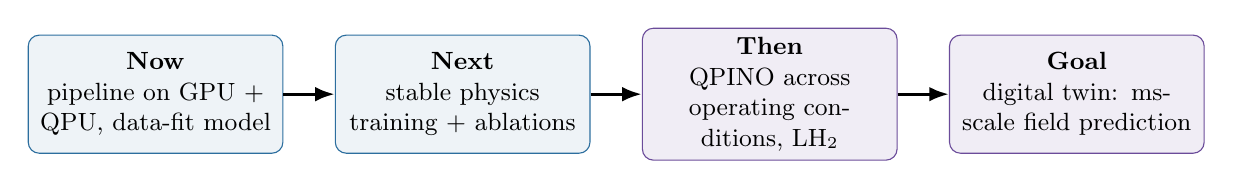
\begin{tikzpicture}[
  font=\small,
  st/.style={rounded corners,draw=cblue,fill=cblue!8,minimum width=3.2cm,minimum height=1.5cm,align=center,text width=3.0cm},
  sq/.style={rounded corners,draw=qpurple,fill=qpurple!10,minimum width=3.2cm,minimum height=1.5cm,align=center,text width=3.0cm},
  arr/.style={-{Latex[length=2.5mm]},very thick}
]
\node[st] (a) at (0,0) {\textbf{Now}\\pipeline on GPU + QPU, data-fit model};
\node[st] (b) at (3.9,0) {\textbf{Next}\\stable physics training + ablations};
\node[sq] (c) at (7.8,0) {\textbf{Then}\\QPINO across operating conditions, LH$_2$};
\node[sq] (d) at (11.7,0) {\textbf{Goal}\\digital twin: ms-scale field prediction};
\draw[arr] (a)--(b); \draw[arr] (b)--(c); \draw[arr] (c)--(d);
\end{tikzpicture}

\vspace{0.4cm}
\begin{columns}[T,onlytextwidth]
\column{0.32\textwidth}
\begin{block}{Data engine}
\footnotesize Agentic CFD (AutoFOAM) generates verified training cases from one prompt.
\end{block}
\column{0.32\textwidth}
\begin{block}{Surrogate}
\footnotesize Hybrid-QPINO trained once, queried across the full process window.
\end{block}
\column{0.32\textwidth}
\begin{block}{Validator}
\footnotesize Physics and benchmark checks before any prediction is trusted.
\end{block}
\end{columns}
\end{frame}

\begin{frame}{Key takeaways}
\begin{enumerate}\setlength{\itemsep}{5pt}
  \item \textbf{Framework:} Fourier features + data re-uploading + a shallow 16-qubit PQC as a trainable feature map, inside a classical physics-informed network.
  \item \textbf{Demonstrated:} the hybrid model fits all five coupled CZ fields (val MSE $1.58\times10^{-4}$) and runs end to end on IBM hardware (500 jobs, 2.05\,M shots, no failures).
  \item \textbf{Learned:} physics weighting must respect field scales; a pressure coefficient of $\sim\!10^5$ can wreck training.
  \item \textbf{Being tested:} faster convergence, better generalisation and lower cost than classical PINN/PINO, via matched ablations.
  \item \textbf{Destination:} QPINO surrogates for crystal growth and LH$_2$ storage as the core of real-time digital twins.
\end{enumerate}
\end{frame}

\begin{frame}{References}
\footnotesize
\begin{itemize}\setlength{\itemsep}{2pt}
  \item Raissi, Perdikaris, Karniadakis, \emph{Physics-informed neural networks}, J.\ Comput.\ Phys.\ (2019).
  \item Rahaman et al., \emph{On the spectral bias of neural networks}, ICML 2019.
  \item Tancik et al., \emph{Fourier features let networks learn high frequency functions}, NeurIPS 2020.
  \item P\'erez-Salinas et al., \emph{Data re-uploading for a universal quantum classifier}, Quantum (2020).
  \item Schuld, Sweke, Meyer, \emph{Effect of data encoding on the expressive power of variational quantum machine-learning models}, PRA (2021).
  \item Wang, Teng, Perdikaris, \emph{Understanding and mitigating gradient pathologies in PINNs}, SIAM J.\ Sci.\ Comput.\ (2021).
  \item Krishnapriyan et al., \emph{Characterizing possible failure modes in PINNs}, NeurIPS 2021.
  \item Li et al., \emph{Physics-informed neural operator for learning PDEs} (2021).
  \item Chapagain et al., \emph{Component-level evaluation of adaptive PINN training for CFD-oriented crystal growth simulation}, NeurIPS 2026 Sim2Science workshop.
  \item Neelan, Seshaditya, \emph{AutoFOAM: the self-refining autonomous OpenFOAM agent}.
  \item Project reports: Hybrid QPINN for Czochralski growth, HPC and IBM Quantum study (2026).
\end{itemize}
\end{frame}

\begin{frame}
\centering
\Large\textbf{Thank you}

\vspace{0.4cm}
\normalsize Questions?

\vspace{0.6cm}
\small Hybrid Quantum AI for accelerating multiphysics simulation
\end{frame}

\end{document}
